\documentclass{article}
\usepackage[utf8]{inputenc}
\title{Lecture 7 probabilistic models - Bayesian methods}
\author{wbg231 }
\date{December 2022}
\newcommand{\R}{$\mathbb{R}$}
\newcommand{\B}{$\beta$}
\newcommand{\A}{$\alpha$}
\newcommand{\D}{\Delta}

\newcommand{\avector}[2]{(#1_2,\ldots,#1_{#2})}
\newcommand{\makedef}[2]{$\textbf{#1}$:#2 }
\usepackage{tikz,graphicx,hyperref,amsmath,amsfonts,amscd,amssymb,bm,cite,epsfig,epsf,url}

\begin{document}

\maketitle

\section{introduction}
\begin{itemize}
\item we have so far done frequentest probabilistic models using MLE 
\item we are going to use Bayesian methods to get some uncertainty around the prediction 
\section{classical stats}
\subsection{parametric family of densities }
\item a parametric family of densities is a set $$\{p(y|\theta):\theta\in \Theta\}$$ this is a set of distributions
\item where $P(y|\theta)$ is a density on a sample space y, and $\theta$ is a parameter in a parameter space $\Theta$
\item  this is a common starting point for Bayesian statistics. 
\subsection*{frequentest statistics}
\item in classical of frequentest statistics we are working with a parametric family of distributions $$\{P(y|\theta: \theta\in \Theta)\}$$
\item however we assume that there is some $\theta_{true}\in\Theta$ which has governed the distribution of our observed data 
\item so if we know $\theta_{true}$ there would be no need for statistics
\item but we can not view the true data generating process, as we only have a finite sample $\mathcal{D}:(y_1...y_n)$ generated independent  and identically distributed  from $P(y|\theta_{true})$
\subsection*{point estimation}
\item one type of statistical problem is point estimation
\item a \textbf{statistic} $s=s(\mathcal{D})$ is any function of our data 
\item \textbf{a point estimator of } \boldmath{$\theta$} is a function of our data $\hat{\theta}=\hat{\theta}
(\mathcal
D)$ for some $\theta\in \Theta$
\item a good point estimate will have $\hat{\theta}\approx \theta_{true}$
\item we want a point estimate to have the following properties
\begin{enumerate}
    \item \textbf{consistency} that is if we think of our point estimate on n data points as $\hat{\theta}_{n}$ then we have $lim_{n\rightarrow\infty}\hat{\theta}_n\rightarrow \theta_{true}$ that is as we get more data our point estimate generally more accurate, that is as we get more data our error gets lower
    \item \textbf{efficiency} formally the efficiency of an unbiased estimator $\hat{\theta}$ of parameter $\theta$ is $e(t)=\frac{\frac{1}{I(\theta)}}{var(\hat{\theta})}$ , where $I(\theta)$ is a measure of the amount about how much our observed data $\mathcal{D}=\{y_1..y_n\}$ tells us about our parameter $\theta$ it related to entropy which is how predicable a variole is effectively. basically this is saying we want our estimator to train well on relatively little data  \href{https://en.wikipedia.org/wiki/Efficiency_(statistics)}{efficency}
\end{enumerate}  
\item maximum likelihood estimators as consistent and efficient under reasonable assumptions
\subsection{coin example}
\item we have a parametric family of mass functions $P(\text{heads}|\theta)=\theta$ for some $\theta\in\Theta:=(0,1)$
\subsection{coin flipping mle}
\item suppose we have dataset $\mathcal{D}=\{H...T\}$ whee we have $n_h$ heads and $n_t $ tails and the flips are iid
\item the likelihood function of our data is then $\mathcal{L}_{\mathcal{D}}(\theta)=P(\mathcal{D}|\theta)=P(y_1...y_n|\theta)
=\Pi_{i=1}^{n}P(y_i|\theta)=(\theta)^{n_h}(1-\theta)^{n_t}$
\item we can max the log likelihood of our data as a function of $\theta$ as $max_{\theta\in \Theta}\ell(\theta)=max_{\theta\in \Theta} n_hlog(\theta)+n_tlog(1-\theta)$
\item we can then see that $\frac{\partial \ell}{\partial \theta}=\frac{n_h}{\theta}-\frac{n_t}{1-\theta}$
\item setting this equal to zero we get $\theta_{mle}=\frac{n_h}{n_h+n_t}$ which is the empirical fraction of heads which makes sense 
\section*{bayesian statistics}
\item in bayesian stats we introduce a prior distribution
\item \textbf{the prior distribution} is defined as $P(\theta)$, and it represents our bellies about how $\theta$ is distributed over the parameter space $\Theta$ prior to seeing any data 
\subsection*{a bayesian model}
\item there are two prices to a bayesian model
\begin{enumerate}
    \item a parametric family of densities $P(\mathcal{D}|\theta\in \Theta)$ that is basically a set of distributions we think our data given the parameter may have 
    \item we alos need our prior $P(\theta):\theta\in \Theta$
    
\end{enumerate}
\item given both of these pieces we can write our joint density $P(\mathcal{D}, \theta)=P(\mathcal{D}|\theta)P(\theta)$ so we have the joint density of our data and the model
\item 
\subsection*{the posterior}
\item \textbf{the posterior distribution} for $\theta \text{ is } P(\mathcal{D}|\theta)$
\item the prior is our belives about the parameter before seeing any data 
\item the posterior represents how we rationally update our beliefs about $\theta$ after seeing our data
\item we can write the posterior as $ P(\mathcal{D}|\theta)=\frac{P(\mathcal
D), \theta)}{P(\theta)}=\frac{P(\mathcal
D|\theta)P(\theta)}{P(\mathcal{D})}$ where we think of both sides as a function of $\theta$ for a fixed dataset $\mathcal{D}$
\item given our data set is fixed $P(\mathcal{D})$ is constant so we can ignore it 
\item so in practice we solve for $P(\mathcal{D}|\theta)P(\theta)$ as we know that $P(\theta|\mathcal{D})\propto P(\mathcal{D},\theta)P(\theta)$
\subsection*{coin flipping bayesian example}
\item supper we have a parametric family of mass functions $P(heads|\theta)=\theta\text{ where }\theta\in \Theta=(0,1)$
\item we need a prior distribution $P(\theta)$ on $\Theta$
\item typically we chose a distribution from the beta family
\subsection*{beta distributions}
\item given we assume our prior is $\theta\sim \text{beta}(\alpha, \beta)$ we know that $P(\theta)\propto \theta^{\alpha-1}(1-\theta)^{\beta -1}$
\item the beta family takes two parameters 
\item given these parameters we get a distribution over $\theta$ but notice that this distribution is independent of our data 
\item the shape of the beta distribution can vary a lot. 
\item 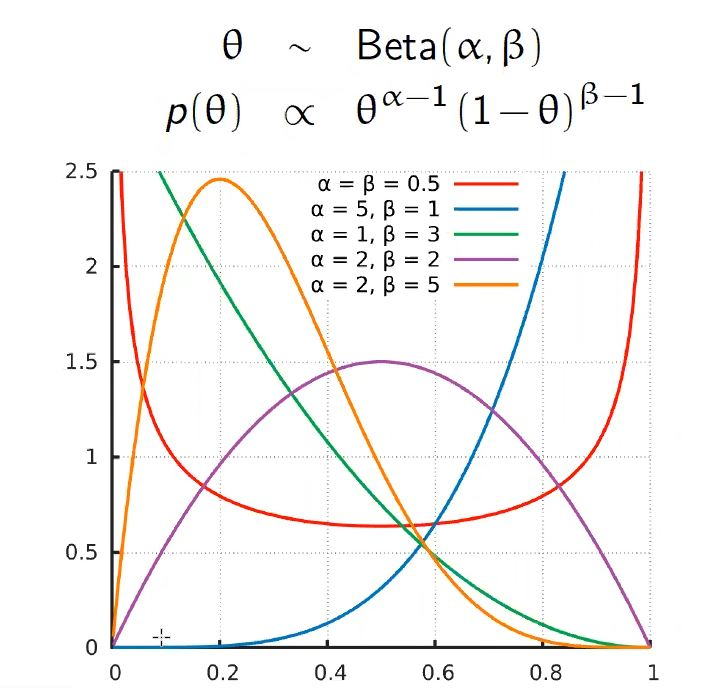
\includegraphics{/home/buzgalbraith/work/school/spring_2023/Machine_Learning_spring_2023/lecture_notes/lecture_7/immages/l7_1.JPG}
\item the beta distribution is nice because it is only defined in 0,1
\item given that $\theta\sim \text{beta}(\alpha, \beta)$
\item $E[\theta]=\frac{\alpha}{\alpha+\beta}$ \href{https://statproofbook.github.io/P/beta-mean.html}{the proof is kind of tedious so i am just going to link it }
\item then we can find the mode of the beta distribution. the mode is the most common value in a pdf that is $argmax_{\theta\in [0,1]}P(\theta)=\frac{\alpha-1}{\alpha+\beta-2}$ 
\item showing the mode is a big less tedious classically just note $P(\theta)=\frac{1}{B(a,b)}\theta^{a}(1-\theta)^b$, then we can take the derivative and solve for $\theta^{*}$
\subsection*{coin flipping prior}
\item lets say that our prior is $\theta\sim beta(c,c)$ where $h=c=t$ that is we are assuming that the likelihood of heads and tails are equal then our mean and mode are both equal to $\frac{1}{2}$
\subsection*{coin flipping posterior}
\item so our likelihood of the deta given  $\theta \text{ is } \mathcal{L}_{\mathcal{D}}(\theta)=P(\mathcal{D}|\theta)=\theta^{n_h}(1-\theta)^{n_t}$
\item then our posterior density is $$P(\theta|\mathcal{D})\propto P(\mathcal{D}|\theta)P(\theta)\propto \theta^{n_h}(1-\theta)^{n_t}\times(1-\theta)^{t}\theta^{h}=\theta^{h-1+n_h}(1-\theta)^{t-1+n_t}$$
\item note that our posterior is in the beta family that is $P(\theta|d)\propto \theta^{h-1+n_h}(1-\theta)^{t-1+n_t}\Rightarrow \theta|\mathcal{D}\sim beta(h+n_h, t+n_t)$
\item as the number of coin flips goes to infinity the prior will matter less as the values of h and t are fixed and $n_h,n_t$ grow, so when we have a lot of data we weigh it quite heavily
\item and when we do not have much data we rely more on our prior
\subsection*{conjugate priors}
\item in this case the posterior was in the same family of distributions as the prior 
\item this makes the math easy 
\item let $\pi$ be a family of posterior distributions on $\Theta$
\item let $P$ a parametric family of distributions on parameter space $\Theta$
\item family of distributions $\pi$ is  \textbf{conjugate} to the parametric model P if $\forall p(\theta) \in \pi$ (that is all priors on $\pi$) the posterior is in $pi$ that is $P(\theta)\in \pi\Rightarrow P(\theta|\mathcal{D})\in \pi$
\item the beta family is conjugate to a bernoulli model 
\item this is not easy to do, but it is nice when it works 
\subsection*{coin flipping concrete example}
\item suppose we a parametric probabilistic model of our coin $P(\text{heads}|\theta)=\theta$
\item and our parameter space is $\theta\in \Theta=[0,1]$
\item and our prior is $\theta\sim beta(2,2)$
\item \includegraphics*{/home/buzgalbraith/work/school/spring_2023/Machine_Learning_spring_2023/lecture_notes/lecture_7/immages/l7_2.JPG}
\item our prior assumes that $\theta$ will be distributed kind of evenly but centered at 0
\subsection*{with data}
\item suppose we have some data, where we saw 75 heads and 60 tails 
\item doing maximum liklyhood estimation we would get $\hat{\theta}_{mle}=.556$
\item using bayesian methods we would get a posterior $\theta|\mathcal{D}\sim beta(77,62)$
\item \includegraphics*{/home/buzgalbraith/work/school/spring_2023/Machine_Learning_spring_2023/lecture_notes/lecture_7/immages/l7_3.JPG}
\item as we can see both estimates are centered at about 55
\item but doing it with bayesian methods we have a distribution of parameters as opposed to just a single estimate of $\theta$
\subsection*{bayesian point estimates}
\item what if want to give a point estimate from our posterior 
\item there are a few common options
\begin{enumerate}
    \item posterior mean $\hat{\theta}=E[\theta|\mathcal{D}]$
    \item maximum a posteriori estimate (MAP) $\hat{\theta}={argmax}_{\theta}P(\theta|\mathcal{D})$ (this is the mode of the posterior )
\end{enumerate}
\subsection*{what else can we do with a prior}
\item we can use it to quantify our uncertainty around the estimate 
\item we could make a credible set for $\theta$ that is an interval $[a,b]:P(\theta\in [a,b]|\mathcal{D})\geq \alpha$ this is effectively bayesian confidence interval
\item we could also select a point estimate using bayesian decisions theory. this requires us to chose a loss function, and chose an action to minimize the expected risk with respect to  
\section{bayesian decision theory}
\item we need the following ingredients 
\begin{enumerate}
    \item parameter space $\Theta$
    \item prior $p(\theta):\theta\in\Theta$
    \item action space A
    \item loss function $\ell:A\times \theta \Rightarrow \mathbb{R}$
\end{enumerate}
\item the output is no longer the parameter it is an action 
\item the posterior risk of an action $a\in A$ (also alled tthe expected loss under the posterior )is $$r(a)=:E[\ell(\theta, a)|\mathcal{D}]=\int \ell(\theta,a)P(\theta|\mathcal{D})d\theta$$
\item so that is more or less looking at a weighted average of our action over all possible values of theta
\item this is more robust as we are only choosing an action a, not a point estimate of our parameter 
\item a byes action $a*=min_{a\in A}r(a)$ the action that minimizes risk, ie the best action 
\subsection*{bayesian point estimation}
\item we have a data set $\mathcal{D}$ genrated by $P(y|\theta)$ for some unkown $\theta\in \Theta$
\item we want a point estiamte for $\theta$
\item we need to chose a prior $P(\theta):\theta\in \Theta$ and loss $\ell(\hat{\theta},\theta)$
\item and our goal is to fund the action $\hat{\theta}$ that minimizes the posterior risk. 
\item the point of this is that bayesian point estimation can be looked with the bayesian decision theory framework
\subsection*{important cases }
\item  squared loss $\ell(\theta-\hat{\theta})=(\theta-\hat{\theta} )^2$ minimizing this gives the $\hat{\theta}=$ posterior mean 
\item zero one loss $\ell(\theta-\hat{\theta})=1(\theta \neq \hat{\theta} )$ minimizing this gives the $\hat{\theta}=$ posterior mode (not a good idea for when $\theta$ is continuous)
\item $\ell(\theta-\hat{\theta})=|\theta-\hat{\theta} |$ minimizing this gives the $\hat{\theta}=$ posterior median 
\subsection*{squared loss example}
\item want to find an action $\hat{\theta}\in \Theta: \hat{\theta}\in argmin_{\theta\in \Theta}\int(\theta-\hat{\theta})^2P(\theta|\mathcal{D})d\theta$
\item we can take the partial of our risk as $\frac{\partial r(\hat{\theta})}{\partial \hat{\theta}}=-2\int(\theta-\hat{\theta})p(\theta|\mathcal{D})d\theta\\
=-2\int\theta P(\theta|\mathcal{D})d\theta+2\theta\int P(\theta|\mathcal{D})d\theta=-2\int \theta P(\theta|\mathcal{D})d\theta+2\hat{\theta}$
\item setting that equal to zero yields $\hat{\theta}=\int\theta P(\theta|\mathcal{D})d\theta=E[\theta|\mathcal{D}]$ 
\item so in other words the optimal action according to squared loss is the posterior mean 
\item all inferences and actions can be taken with only a prior and loss function 
\item in the bayesian approach we do not need to justify our estimator, we just need to specify our family of distributions and the prior
\item try to use the conjugate prior when you can 
\item for a lot of data the prior does not matter very much 
\section*{recap of conditional probabilistic models}
\subsection*{conditional probabilistic models}
\item input space X
\item outcome space y 
\item action space $A=\{P(y)|\text{p is a probablity distribution on y }\}$
\item hypothesis space $\mathcal{F}$ contains prediction function mapping $f:X\rightarrow A$
\item prediction function $f\in \mathcal{F}:f(x)$ produces a distribution on y
\item a parametric family of conditional densities is a set $\{P(y|x,\theta):\theta\in \Theta\}$
\item where $P(y|x,\theta)$ is a density on the outcome space y for each x in input space and $\theta$ is a parameter in the parameter space 
\item the action space here is a probability distribution not just a decision
\subsection*{likelihood function}
\item we can as always find our likelihood function given our data set $P(\mathcal{D}|x_1...x_n, \theta)=\Pi_{i=1}^{n}P(y_i|x_i,\theta)$
\item the mle estimator is the the $\hat{\theta}_{mle}=argmax_{\theta\in \Theta}\mathcal{L}_{\mathcal{D}}(\Theta)$
\item the corresponding prediction function is $f(x)=P(y|x,\hat{\theta}_{mle})$
\section*{bayesian condtiional models }
\item input space $X= \mathbb{R}^{D}$ outcome space $Y=\mathbb{R}$
\item parametric family of distributions $\{P(y|x,\theta):\theta\in \Theta\}$
\item prior $P(\theta):\theta\in \Theta$ (so we have added a prior )
\item the posterior is $P(\theta|\mathcal{D}, X)\propto P(\mathcal{D}|\theta)P(\theta)=\mathcal{L}_{\mathcal{D}}(\theta)p(\theta)$
\item we don't worry about the denominator in this case because the dataset is fixed so we can just look at the proportional 
\item we can use bayesian decisions theory to derive point estimates, we have a few choices for how we do this. also depends on our loss function 
\subsection*{bayesian prediction function}

\item we want to find a prediction function that takes input $x\in X$ and produces a distribution on Y
\item in the frequentest approach we chose a conditional family of probability distributions (hypothesis space) and select one conditional probability from the family based on some rule like the mle
\item in Bayesian setting we chose a parametric family of conditional densities $$\{P(y|x,\theta):\theta\in \Theta\}$$ and a prior distribution $P(\theta):\theta\in \Theta$
\item with a bayesian model how do we predict a distribution on y for input x 
\item we do not need to make a discrete selection from the hypothesis space: we can maintain some uncertainty
\subsection*{prior predictive distribution}
\item suppose we have not yes observed any data 
\item in teh Bayesian setting we can still produce a prediction function 
\item call \textbf{the prior predictive distribution} $$x\rightarrow P(y|x)=\int P(y|x,\theta)p(\theta)d\theta$$ 

\item this is an average of all conditional densities in our family weighted by the prior. 
\item so we are considering all possible $\theta$ and we get out a $P(y|x)$
\subsection*{posterior predictive distribution}
\item after seeing our data set $\mathcal{D}$
\item the posterior predictive distribution is given by  $$x\rightarrow P(y|x,\mathcal{D})=\int P(y|x,\theta)P(\theta|\mathcal{D})d\theta$$
\item this is an average of all conditional densities in our hypothesis space weighted by the posterior distribution , so we are again considering all $\theta$
\item ewe have not chosen a particular $\theta$ we consider all and just weighted by there likelihood
\subsection*{comparing to the frequentest approach}
\item in bayesian stats we have two distributions on $\Theta$ the prior, and the posterior $P(\theta|\mathcal{D})$
\item there distributions are over parameters corresponding to the distribution on the hypothesis space so, what we get out is a distribution on the hypothesis space
\item in the frequentest approach we just pick one $\hat{\theta}$ that we think is best 
\item in the bayesian approach we weight over all possible outcomes 
\subsection*{what if we don't want a full distribution on y }
\item once we have a predictive distribution $P(y|x,\mathcal{D})$ we can generate a single prediction
\item there are many choices depending on what loss we want to minimize
\section*{gaussian regression example}
\subsection*{example in 1 dimension}
\item pick up at 47 minutes 
\end{itemize}
\end{document}
